\section{Implementation}
\label{sec:implementation}
This section describes the implementation of the \projecttitle library based on the algorithm presented in~\secref{algorithms}. We implemented \projecttitle as a dynamically linkable shared library for the GNU/Linux OS that can be loaded and linked  at runtime for {\tt POSIX} threads (replacing the \pthreads library). The application executables can simply link the library (without any recompilation) either using {\tt LD\_PRELOAD} or the {\tt -rdynamic} flag, specifying the path of the \projecttitle library.   Our implementation is based on the existing Dthreads library~\cite{dthreads-sosp-2011}, and therefore reuses some of its implementation mechanisms, as highlighted throughout this description.


The architecture of \projecttitle (shown in Figure~\ref{fig:basicSystem}) consists of three main components: memory system, recorder, and OS support.  We next describe each component in detail.

\begin{figure}[t]

\centering
      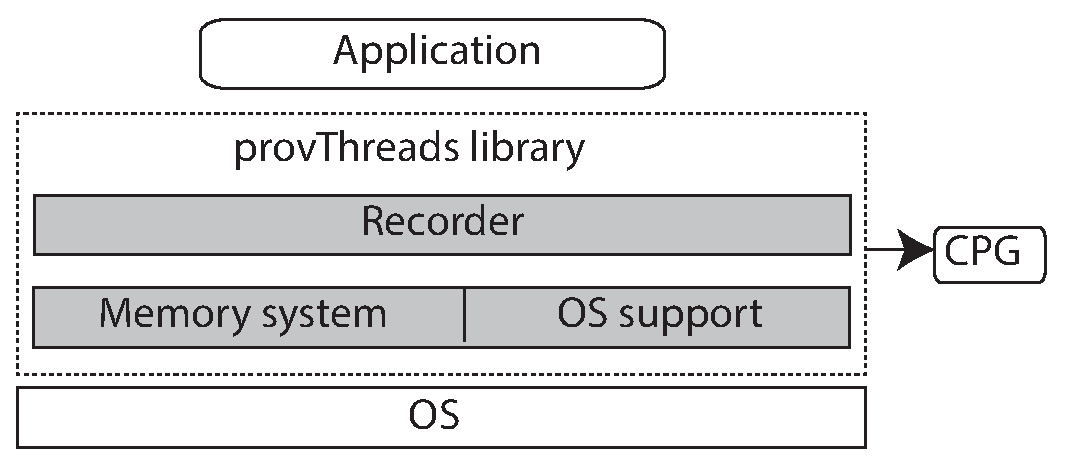
\includegraphics[scale=.4]{figure/System-basic-architecture}
  \caption{\projecttitle architecture. (System components are shown in grey boxes.)}
   
  \label{fig:basicSystem}

\end{figure}



\subsection{Memory System}


\myparagraph{Memory protection} A central challenge of the implementation of the algorithm is keeping track of the data dependencies for shared-memory accesses by all possible interleaving threads. Since monitoring every load and store to each memory word would be too costly, we instead rely on the OS's (hardware-assisted) page fault mechanism to keep track of reads and writes at the granularity of memory pages.

To derive the read and write sets during thunk execution,  \projecttitle~uses standard memory protection  mechanism and signal handlers. In particular, \projecttitle protects the address space using {\tt mprotect(PROT\_NONE)} at the beginning of each thunk. This forces a trap (and the corresponding OS signal) the first time a page is read or written to in a given thunk. The respective signal handler, which is implemented by the \projecttitle library, records the information about the access, and also resets the protection bits so that subsequent accesses to the same page by the same thread in the same thunk can proceed without generating a trap, and therefore avoid a
latency penalty.  

However, a naive page protection mechanism raises an important problem because all threads in a process share the same virtual memory
structures (namely the TLB and page table entries with the respective protection bits). This makes it difficult to keep track of which
threads are responsible for which memory accesses or to enforce different protections for different threads. Otherwise, we need to re-protect the page after serving every load and store instruction causing a large number of page faults.
%(E.g., an access to a given memory location may or may not be the first access in a thunk depending on which thread is performing the access.) 
To address this problem, \projecttitle implements threads as separate
processes (an idea originally proposed by Grace~\cite{grace-oopsla-2009} and also used in Dthreads~\cite{dthreads-sosp-2011}).

\myparagraph{Private address space} \projecttitle  implements threads as separate processes thus allowing each thread has its own private address space and control over the virtual
memory structures.   This gives us the ability to manipulate the page protection of threads individually while providing a simple way to implement the release consistency memory
model. In particular, \projecttitle uses the {\tt clone} system call to fork off a new process on {\tt pthread\_create()}. The process that implements the newly created thread (i.e., the child process) already
shares parts of the execution context with the parent process (which implements the calling thread) such as file descriptors and signal handlers. 


But this raises a new problem, which is that, unlike threads, processes do not share their address spaces. We address this by taking advantage of the RC memory model we defined for \projecttitle, where threads share the updates only at synchronization points.  To implement the RC memory model, we use shared memory commit of Dthreads that allows threads to communicate at well-defined synchronization points.


\myparagraph{Shared memory commit} This shared memory commit is implemented using memory mapped files. In
particular, the virtual address ranges for the shared portions (globals and heap) of
the address space are mapped to memory mapped files, which are managed by the
\projecttitle library. These address ranges correspond to the heap and
the static (i.e., globals) regions.  During thread creation,
\projecttitle marks these address ranges as a private copy-on-write
mapping (using {\tt MAP\_PRIVATE} in {\tt mmap()}). The effect of this
is that whenever the child thread tries to write to a memory location,
the OS makes a thread-private copy of the memory page containing the
modification.  At synchronization points, the thread computes a {\em diff}
for each dirty page by performing a byte-level comparison between the
dirty page and the shared page. The deltas are then atomically
copied to the shared memory page; if there are overlapping writes
to the same memory location we resolve them using a last-writer wins policy.
\subsection{Recorder}

\subsection{OS Support}